\def\mytitle{Coursework Report}
\def\mykeywords{Algorithms, and, data, structures, coursework, report, checkers, draughts, game}
\def\myauthor{William Daglish}
\def\contact{40216858@napier.ac.uk}
\def\mymodule{Algorithms and Data Structures (SET09117)}
\documentclass[10pt, a4paper]{article}
\usepackage[a4paper,outer=1.5cm,inner=1.5cm,top=1.75cm,bottom=1.5cm]{geometry}
\usepackage{graphicx}
\graphicspath{{images/}}
%colour our links, remove weird boxes
\usepackage[colorlinks,linkcolor={black},citecolor={blue!80!black},urlcolor={blue!80!black}]{hyperref}
%Stop indentation on new paragraphs
\usepackage[parfill]{parskip}
%% Arial-like font
\IfFileExists{uarial.sty}
{
    \usepackage[english]{babel}
    \usepackage[T1]{fontenc}
    \usepackage{uarial}
    \renewcommand{\familydefault}{\sfdefault}
}{
    \GenericError{}{Couldn't find Arial font}{ you may need to install 'nonfree' fonts on your system}{}
    \usepackage{lmodern}
    \renewcommand*\familydefault{\sfdefault}
}
%Napier logo top right
\usepackage{watermark}
\usepackage{lipsum}
\usepackage{xcolor}
\usepackage{listings}
\usepackage{float}
\usepackage{wrapfig}
%tone down the line spacing after section titles
\usepackage{titlesec}
\usepackage{amsmath}

\titlespacing{\subsection}{0pt}{\parskip}{-3pt}
\titlespacing{\subsubsection}{0pt}{\parskip}{-\parskip}
\titlespacing{\paragraph}{0pt}{\parskip}{\parskip}
\newcommand{\figuremacro}[5]{
    \begin{figure}[#1]
        \centering
        \includegraphics[scale=#5]{#2}
        \caption{\textbf#4}
        \label{#3}
    \end{figure}
}

\lstset{
	escapeinside={/*@}{@*/}, language=C++,
	basicstyle=\fontsize{8.5}{12}\selectfont,
	numbers=left,numbersep=2pt,xleftmargin=2pt,frame=tb,
    columns=fullflexible,showstringspaces=false,tabsize=4,
    keepspaces=true,showtabs=false,showspaces=false,
    backgroundcolor=\color{white}, morekeywords={inline,public,
    class,private,protected,struct},captionpos=t,lineskip=-0.4em,
	aboveskip=10pt, extendedchars=true, breaklines=true,
	prebreak = \raisebox{0ex}[0ex][0ex]{\ensuremath{\hookleftarrow}},
	keywordstyle=\color[rgb]{0,0,1},
	commentstyle=\color[rgb]{0.133,0.545,0.133},
	stringstyle=\color[rgb]{0.627,0.126,0.941}
}

\thiswatermark{\centering \put(336.5,-38.0){
\includegraphics[scale=0.8]{logo}} }
\title{\mytitle}
\author{\myauthor\hspace{1em}\\\contact\\Edinburgh Napier University\hspace{0.5em}-\hspace{0.5em}\mymodule}
\date{}
\hypersetup{pdfauthor=\myauthor,pdftitle=\mytitle,pdfkeywords=\mykeywords}
\sloppy
% #######################################
% ########### START FROM HERE ###########
% #######################################
\begin{document}
    \maketitle
\section{Introduction}
The aim of this coursework was to design and code a Checkers/Draughts game using any methods \& coding language that was desired.
\newline
\newline
Game such as Checkers, TicTacToe, etc. require the use of specific data structures to produce things like the game boards and player moves/pieces.
By undergoing this project, I will have to demonstrate my knowledge of different data structures and show how they can be implemented to aid in completion of certain tasks.
\newline
\newline
Additionally, there are several functions that my game is required to have, such as: undo/redo moves, watch replay of old games, and an AI (computer) player.
These functions can be accomplished with algorithms that make use of the data structures I have chosen to use.
\newline
\newline
As a bonus, my aim was to get these functions working within a GUI environment. This will obviously be more visually appealing and more user friendly than a console/text based game.
I prefer the GUI to be clean and clear, with only the required interface buttons and labels etc.

\textbf{Keywords -- }{\mykeywords}
    
\section{Software Design}
{
The code language I decided to use for the creation of my game was Java, as this is a language I wanted to get more use out of and try and improve my knowledge on.
\newline
\newline
The main feature of the game was a playable game board, and this is where the main data structure comes into place. The obvious choice was the use of a 2D multidimensional array, as it is immutable and can be thought of quite simply as a table of objects. (Fig 1)
\figuremacro{H}{Fig1}{}{ - Multidimensional Array Example}{0.8}
\newpage
To make the array user interactive, it is an array of type "JButton", a button used in a Java Swing application. (Fig 2) Each button in the array is a position (X \& Y coordinate) on the game board. 
\begin{wrapfigure}{l}{0.25\textwidth} %this figure will be at the left
    \centering
    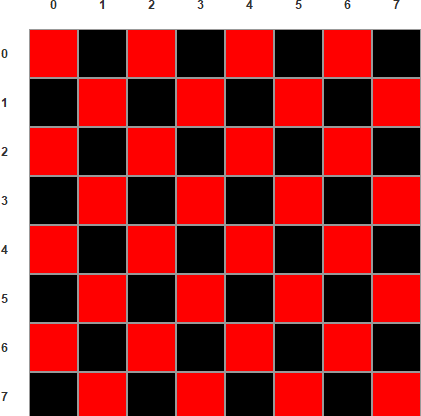
\includegraphics[width=0.25\textwidth]{Fig2}
\label{fig:}
\caption{ - Multidimensional JButton Array for Board}
\end{wrapfigure}
\newline
When loading a new game, each of these positions can be assigned a Checker Piece where required. The checker pieces themselves are "Icons", so when a piece is loaded at coordinate 2,4 for example, that square is assigned an icon, e.g. Black Checker. (Fig 3)
Each button is then set with an ActionListener which handles clicks.
\qquad
\figuremacro{H}{Fig3}{}{ - Pieces (Icons) Loaded to the Board}{0.6}
\qquad
\\
}
To start a new game, quit a game, or access some other functions, the user can interact a menu which is implemented with a "JMenuBar". (Fig 4 \& 5) The different items in the menu make use of specific "ActionEvents" and call methods which setup a game, clear a game, and carry out the additional functions specified in my introduction (undo, redo etc.).

\figuremacro{H}{Fig4}{}{ - Choosing a Game Type}{0.6}
\figuremacro{H}{Fig5}{}{ - Different Game Functions}{0.6}
\newpage
Probably the most complicated part of this project was to setup and restrict the moves a user could make.
\newline
\\
The actual legal moves and jumps themselves are monitored by methods in the Move class.
When a user clicks on a square to try and move a piece, the ActionListener passes these source and destination coordinates to the makeMove/makeJump methods in this class.
The method then checks if it can move/jump (Listing 1), if it is a legal move then it returns true and the piece is moved.
\newline
\\
If the move is not legal then an "Invalid Move" message is returned to the user. All messages like this are shown next to the Menu bar with the use of a "JLabel".

\begin{lstlisting}[caption = canJump Algorithm - Checking if a Jump is Legal]
public static boolean canJump(int player, int fromX, int fromY, int jumpX, int jumpY, int toX, int toY)
{
	if (toY < 0 || toY >= 8 || toX < 0 || toX >= 8) 
	{
		return false; //Move is off the board.
	}
	if (Board.boardSquares[toX][toY].getIcon() == Piece.BLACKCHECK || Board.boardSquares[toX][toY].getIcon() == Piece.REDCHECK ||
			Board.boardSquares[toX][toY].getIcon() == Piece.BLACKKING || Board.boardSquares[toX][toY].getIcon() == Piece.REDKING)
	{
		return false; //Move already contains a piece.
	}
	if (player == ActionClicks.REDPLAYER)
	{
		if (Board.boardSquares[fromX][fromY].getIcon() == Piece.REDCHECK && toY < fromY)
		{
			return false; // Regular red piece can only move up.
		}
		if (Board.boardSquares[jumpX][jumpY].getIcon() != Piece.BLACKCHECK && Board.boardSquares[jumpX][jumpY].getIcon() != Piece.BLACKKING)
		{
			return false; // There is no black piece to jump.
		}
		return true; // The jump is legal.
	}
	else
	{
		if (Board.boardSquares[fromX][fromY].getIcon() == Piece.BLACKCHECK && toY > fromY)
		{
			return false; // Regular black piece can only move down.
		}
		if (Board.boardSquares[jumpX][jumpY].getIcon() != Piece.REDCHECK && Board.boardSquares[jumpX][jumpY].getIcon() != Piece.REDKING)
		{
			return false; // There is no red piece to jump.
		}
		return true; // The jump is legal.
	}
}
\end{lstlisting}

\qquad

The other functions in this game such as the AI player, the undo/redo methods and the replay, all make use of a "List" data structure.
\newline
This is used as the number of items that are being stored will vary a lot throughout the game, so the data structure needed to be mutable.
\newline
All pieces that are owned by the AI Player are stored in a List at the start of every move (Listing 2), so that the AI can try and move from one of these locations.
\qquad

\begin{lstlisting}[caption =  - getAIPieces Method - Fill a List with Coordinates of Any AI Controlled Pieces]
public static void getAIPieces()
{
	for(int i=0; i<8; i++)
	{
		for(int j=0; j<8; j++)
		{
			if(Board.boardSquares[j][i].getIcon() == Piece.REDCHECK || Board.boardSquares[j][i].getIcon() == Piece.REDKING)
			{
				//Search for pieces that are red and save their X & Y coords to list
				computerPieces.add(Integer.toString(j) + "" + Integer.toString(i));
			}
		}
	}
}
\end{lstlisting}

\newpage

The algorithm that makes the AI player move makes use of the Random function (Listing 3) in Java, calling a random piece from the list and calling a number between 0 - 3, with each number pointing to a specific move/jump direction.
\newline
If this move is not possible then the number simply increments and tries again. After a successful move, the AI Pieces list is cleared so that it can be updated next turn.

\begin{lstlisting}[caption =  - Methods for AI - Getting a Random Source \& Destination Coordinate]
private static void getRandomPieceSource()
{
	//Get a random x & y source coordinate from the list of controlled pieces
	Random randomPieceSource = new Random();
	randomSource =  computerPieces.get(randomPieceSource.nextInt(computerPieces.size()));
}

public static void getRandomPieceDest()
{
	//Random int from 0-3
	Random randomPieceDest = new Random();
	randomDest = randomPieceDest.nextInt(4) + 0;
}
\end{lstlisting}

\qquad

Finally, the History class makes use of a List to store the moves that are made during a game (Listing 4).
\newline
These elements in the list contain the source and destination coordinates of each move. This allows the user to call the undo/redo functions.

\begin{lstlisting}[caption =  - Methods for History List - Stores the Move Coordinates to the List]
private static List<String> historyOfMoves = new ArrayList<>();

public static void addToHistory()
{
	historyOfMoves.add(Integer.toString(Move.originX));
	historyOfMoves.add(Integer.toString(Move.originY));
	historyOfMoves.add(Integer.toString(Move.destinationX));
	historyOfMoves.add(Integer.toString(Move.destinationY));
	historyOfMoves.add(System.lineSeparator());
}
\end{lstlisting}

\newpage
Not only can a user undo/redo moves but they can also save a particular game and load it later to continue play or watch a replay of all the moves carried out.
\newline
If a user chooses to save a game, the current list of moves taken is stored to a text file, line by line. This can later be read using a buffered reader.
\newline
\\
If the file is selected to "Watch a Replay", then the buffered reader is loaded into a new thread and the thread "sleeps" for 1 second after each move. (Listing 5) This allows the user to easily see the game being played out.
\newline
\\
The reason that multi-threading is being used for this algorithm is that it prevents any issues the "Sleep" method causes when used in conjunction with a Swing application.

\begin{lstlisting}[caption =  - Method for Action Replay - Loads the Selected File and Plays Out Each Move with a 1 Second Delay]
public static void openHistoryThread()
{
    new Thread(new Runnable()
    {
		@Override
		public void run() {
			try
			{
				readFromHistory();
			}
			catch (InterruptedException e)
			{
				e.printStackTrace();
			}
		}
    }).start();
}

private static void readFromHistory() throws InterruptedException
{
	Piece.setupNewGame();
	Thread.sleep(1000);
    try (BufferedReader br = new BufferedReader(new FileReader(selectedFile)))
    {
        String line;
        while ((line = br.readLine()) != null)
        {
        	int originX = Integer.parseInt(line.substring(0,1));
        	System.out.println(originX);
        	int originY = Integer.parseInt(line.substring(1,2));
        	System.out.println(originY);
        	int destinationX = Integer.parseInt(line.substring(2,3));
        	System.out.println(destinationX);
        	int destinationY = Integer.parseInt(line.substring(3));
        	System.out.println(destinationY);
    		if((destinationX == originX + 2) || (destinationX == originX - 2))
    		{
        		Move.makeJump(originX, originY, destinationX, destinationY);
        		ActionClicks.resetBorderHighlights();
        		System.out.println("Jumping: " + originX + " " + originY + " " + destinationX + " " + destinationY);
        		Thread.sleep(1000);
    		}
    		else
    		{
        		Move.makeMove(originX, originY, destinationX, destinationY);
        		ActionClicks.resetBorderHighlights();
        		System.out.println("Moving: " + originX + " " + originY + " " + destinationX + " " + destinationY);
        		Thread.sleep(1000);
    		}
	    }
   	}
   	catch (FileNotFoundException e)
   	{
   		e.printStackTrace();
		System.err.println("Error: File can't be read.");
	}
    catch (IOException e)
    {
    	e.printStackTrace();
    	System.err.println("Error: File can't be read.");
    }
}
\end{lstlisting}
\newpage

\section{Enhancements}
Possible improvements that could be made to this game would be the use of "Minimax" algorithms for the AI Player.
\newline
These would help make the AI a more effective player by letting it evaluate each of its current possible moves by determining whether that move will end up resulting in a win.
\newline
\\
Another possible feature that could be added to this game would be the option to select different international rule sets. Certain countries use different rule sets to the ones that are used in this game.

\section{Critical Evaluation}
The main feature that I feel works well is the actual use of a GUI over a text based game.
\newline
As I had initially planned, I feel that it makes the game more user friendly and more interesting to play.
\begin{wrapfigure}{r}{0.35\textwidth} %this figure will be at the left
\centering
  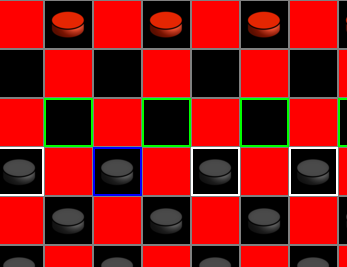
\includegraphics[width=0.25\textwidth]{Fig6}
  \label{fig:}
\caption{ - Highlighting Possible Moves \& Selected Piece}
\end{wrapfigure}
\newline
The buttons worked well for moving different pieces around the board, and the algorithms which determine jumps/moves that are legal also highlight these possible moves (Fig 6). This again makes the game more user friendly.
\\
I also feel that the AI makes quite an effective player. Even though I didn't use a minimax algorithm, the fact that the AI moves are completely random means that they are unpredictable.
\newline
This prevents the user from guessing how the game will play out.

\section{Personal Evaluation}
This project has been very challenging in some areas, particularly in getting the actual gameplay and movement working. It has however forced me to think of different ways I can accomplish the tasks set out in the specification, and as described, what data structures I will need to use and why.
\newline
\\
I also found that creating a game was more interesting and fun than some other projects I have been given in the past. Overall I think that I have managed to completed the majority of the tasks set out in the original coursework specification, and I am fairly happy with my final product.

\end{document}